\subsubsection{H-Brücke}
\label{subsubsec:H-Brücke}

Das Bindeglied zwischen Kraft (Motor) und Steuersignalen wird von der H-Brücke gebildet. Durch Laden-/Entladen der MOSFET-Gates wird die Spannung am Motor kommutiert.

\paragraph{Schema}\mbox{}

Der Schaltungsaufbau ergibt sich durch den dreiphasigen Aufbau des BLDCs. Es werden so drei Stränge gebildet, woran jeweils eine Spule verbunden wird. Der Energiefluss führt dabei über einen Strommesswiderstand. Die Eingänge der H-Brücke werden zusätzlich mit Stützkondensatoren bestückt, um eine saubere 48V-Netzspannung zu gewährleisten.

\begin{figure}[H]
	\centering
	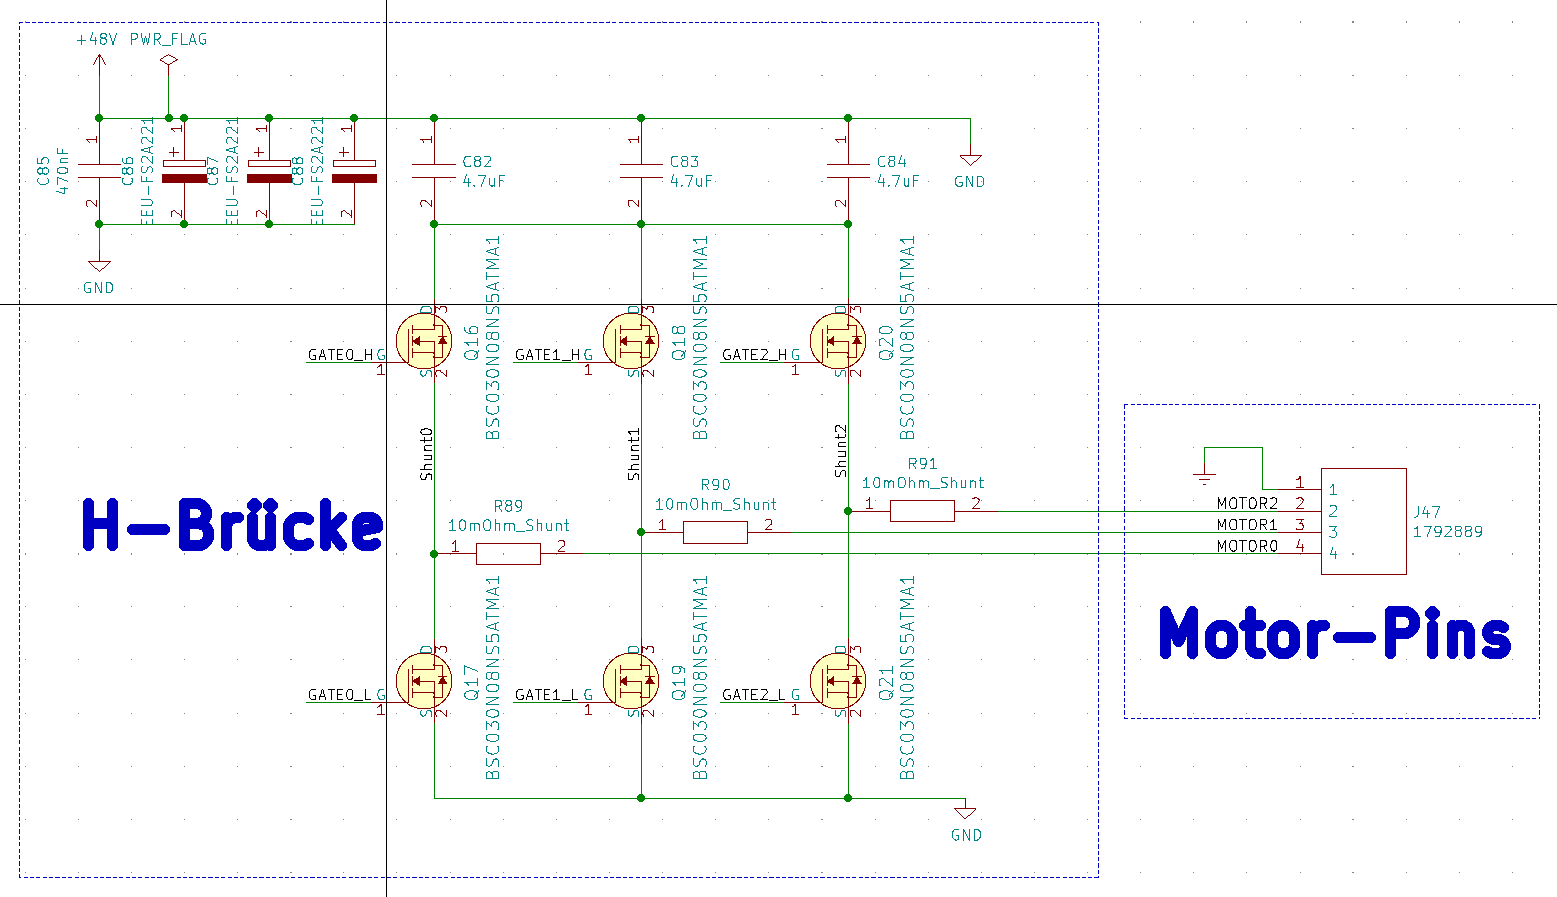
\includegraphics[width=\textwidth]{graphics/Schema_H_Bruecke_und_BLDC}
	\caption{Schema H-Brücke.}
	\label{fig:Schema_H_Bruecke_und_BLDC}
\end{figure}

\paragraph{Funktionsbeschrieb der Schaltung}\mbox{}

Für die Messung des Stromes wird ein \textbf{Shunt} in Serie mit der Spule des BLDC-Motors geschaltet.
Die Shunts für die Strommessung R89 - R91 sind in Abbildung \ref{fig:Schema_H_Bruecke_und_BLDC} zu sehen. Durch den fliessenden Strom liegt eine Spannung über dem Shunt an, welche dann vom Gate-Treiber verstärkt wird und aufbereitet an den FOC-Treiber ausgegeben wird. Die Dimensionierung der Widerstände ist an den Maximalstrom plus 25-50\% Reserve angelehnt. Im Falle des AKM22h sind dies 5A. Aus dem Datenblatt ist einer Tabelle zu entnehmen, wie gross der Shunt bei gegebenem Strom sein muss. Die Schaltung für den PartyMixer wird auf 10A ausgelegt. Gemäss der Tabelle muss der Widerstand 10m\textOmega\ sein, was bedingt, dass ein Verstärkungsfaktor der Phasenströme von 10x eingestellt wird. Die zugehörige Tabelle aus dem Datenblatt ist im Anhang Kapitel \ref{Appendix:Shunt} zu finden \cite[S.31]{trinamicmotion_control_gmbh__co_kg_tmc6200_2019}.

Die Eingangsspannung der gesamten H-Brücke wird mit den \textbf{Stützkondensatoren} C85-C88 in Abbildung \ref{fig:Schema_H_Bruecke_und_BLDC} geglättet.
Bei C86-C88 handelt sich um Low-ESR Kondensatoren, jeweils einen pro Phase.
Die Kondensatoren C82-C84 sind Stützkondensatoren, welche direkt zwischen Ein- und Ausgang eines H-Brücken-Strangs, nahe der MOSFETs platziert sind.

Die \textbf{MOSFETs} Q16-Q21 in Abbildung \ref{fig:Schema_H_Bruecke_und_BLDC} bilden die eigentliche H-Brücke. Sie Schalten den Leistungsfluss gemäss den Gate-Ctrl-Signalen. Sie sind für 100A Nennstrom und 100V Sperrspannung ausgelegt. Die Gate-Source-Spannung beträgt $\pm$20V.

Der Sockel J47 in Abbildung \ref{fig:Schema_H_Bruecke_und_BLDC} bildet die Schnittstelle zwischen Leiterplatine und Motorleitungen. Der Motor wird direkt auf die vorgesehenen Anschluss-Pins geführt. Obwohl die Versorgungsspannung unterhalb der maximalen Berührungsspannung liegt, ist für den Fall eines Defekts im Motor zur Personensicherheit ein Pin für die Erdung des Motorengehäuses vorgesehen.